\subsection{An\'alisis de Tiempo de C\'omputo}
\label{subsec:exp4}
\begin{LaTeXdescription}
    \item[Objetivo] Analizar la complejidad temporal del m\'etodo.

    \item[Hip\'otesis] Proponemos que el tiempo de c\'omputo por iteraci\'on
        para una instancia y $\epsilon$ fijos ser\'a siempre el mismo para todo
        $\alpha$. Tambi\'en proponemos que el tiempo de c\'omputo por interación
        para $\epsilon$ fijo ser\'a el mismo para \textbf{toda instancia} (sin
        importar tama\~no, cantidad de ejes, etc).

    \item[Proposici\'on] De los experimentos previo hemos llegado a la
        conclusi\'on de que a mayor $\alpha$, mayor cantidad de iteraciones
        ser\'an necesarias para converger, lo cual implica inmediatamente un mayor tiempo
        de c\'omputo requerido. La pregunta ideal a responder ser\'ia ''cu\'anto
        tiempo'', pero
        tambi\'en concluimos previamente que la cantidad de iteraciones es
        dependiente (entre otros factores) de la instancia de entrada. Con lo
        cual, responder a esta pregunta en el contexto de este trabajo es
        imposible sin una cota te\'orica para la cantidad de
        iteraciones (que ni siquiera sabemos si existe). En cambio, lo que si podemos analizar es
        si el tiempo de c\'omputo \textbf{por iteraci\'on} es el mismo para toda
        instancia, sin importar el $\epsilon$\footnote{M\'as all\'a de para nuestros
        experimentos lo estemos dejando fijo.} o $\alpha$. Analizamos entonces
        si el tiempo por iteraci\'on var\'ia seg\'un
        la densidad de la instancia inicial, y a su vez si varía para distintos
        valores de $\alpha$.

    \item[M\'etodo de Experimentaci\'on] Tomamos 2 instancias de tama\~no
        mediano-grande, con una diferencia relativa de densidad entre ellas
        significativa. Luego resolvemos cada instancia con PageRank 10 veces
        para $\alpha = 0 0.1 0.2 \dots 0.9$\footnote{Totalizando un total de 200
        corridas del m\'etodo (10 corridas para 10 valores de $\alpha$ para 2
        instancias distintas).}.  Tomamos entonces para cada instancia y
        $\alpha$ fijos, el promedio de los tiempos de c\'omputo. Por \'ultimo,
        calculamos el tiempo de c\'omputo por iteraci\'on dividiendo este
        promedio por la cantidad de iteraciones totales que necesit\'o el
        m\'etodo para converger.

    \item[Resultados, an\'alisis y discusi\'on]
\end{LaTeXdescription}

\begin{figure}[!h]
    \centering
    \subfloat[][Tiempo por Iteraci\'on promedio vs Densidad del Grafo]{
        \label{subfig:exp4_den}
        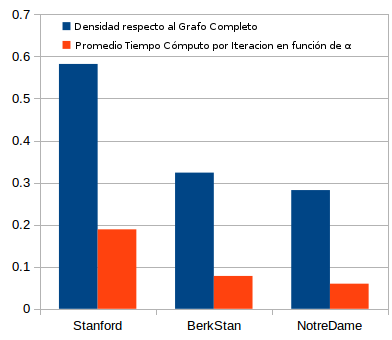
\includegraphics[width=.45\textwidth]{exp4_tiempo_vs_densidad.png}
    }
    \subfloat[][Tiempo por Iteraci\'on en funci\'on de $\alpha$]{
        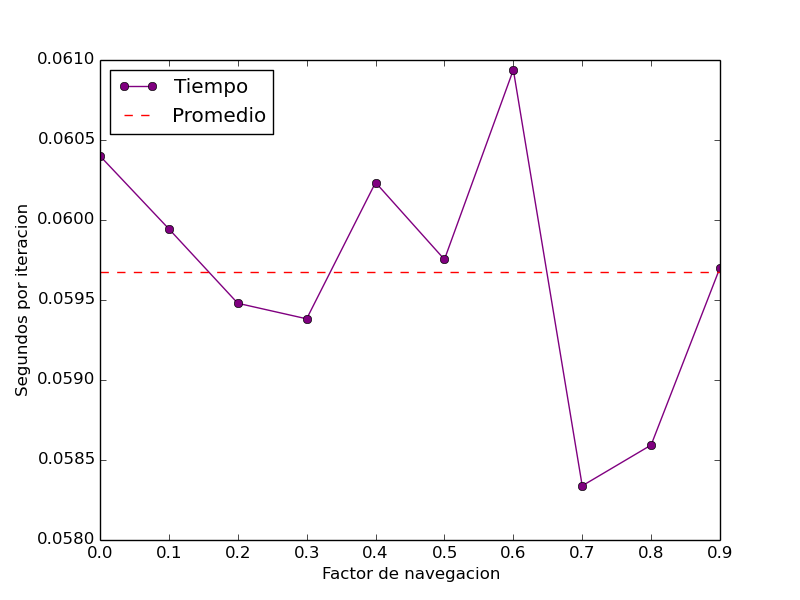
\includegraphics[width=.55\textwidth]{exp4_tiempo_por_iteracion_notredame.png}
        \label{subfig:exp4_tiempo_iteracion}
    }
    \caption{An\'alisis de Tiempo de C\'omputo en funci\'on de $\alpha$ y
        Densidad del Grafo}
\end{figure}
